\documentclass{article}
\usepackage[utf8]{inputenc}
\usepackage[Frech]{babel}
\usepackage{graphicx}

\title{Projet 5}
\author{LEBOBE timothé}
\date{19 juin 2020}

\begin{document}

    \maketitle
    \tableofcontents

    \section{Biographie de Fibonacci}
        Fibonacci est né à Pise mais il étudie en grande partie en Algérie à Bougie, une ville d'influence marchande et intellectuel.
        Il étudie les travaux algébriques du Persan Al-Khwarizmi et de l'Egyptien Abu Kamil. Il voyage beaucoup en aidant son père qui est
        notaire et marchand. Ces voyages lui permettent de rencontrer d'autre mathématiciens. De 1198 à 1228, il compile ses conaissance 
        en écrivant des ouvrages. Après 1228, sa vie est peu connu, en 1241, il a perçut un salaire de la part de la république de Pise
        pour comptabilité. Il meurt peut après.\\
        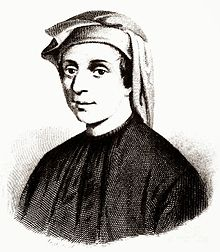
\includegraphics{Fibonacci_portrait.jpg}
\end{document}
